\subsection{Encryption} \label{section:counter-replace-encryption}
way to replace unary license verification is to apply encryption since it outcome is not guessable anymore
two important quesions have to be asks
what will be target of encrypion
where will the eky be retrieved and where is it stored, difficult since online offline

\subsubsection{Encryption} \label{subsubsection:counter-replace-encryption-content}
Encryption can be applied on different levels inside the application.
It has to be decided to which extend it should be applied.
The thesis introduces three different approaches on encryption.

\subsubsection{Resource Decryption} \label{subsection:counter-replace-encryption-content-resource}
The first approach is to apply encryption on the application's static resources.
This includes the application's hard coded strings as well as image assets.
Whenever a resource is used, it has to be decrypted first.
The increase in security comes at the cost of decreased performance.
As long as application critical strings, like server addresses are encrypted, the application is unable to work.
In case no critical strings are present, the application will work as usual, but the user experience will be not sufficient because all strings are still encrypted and thus have no meaning.
Figure~\ref{fig:encryptionResource} shows the abstract implementation of resource decryption.
\begin{figure}[h]
    \centering
    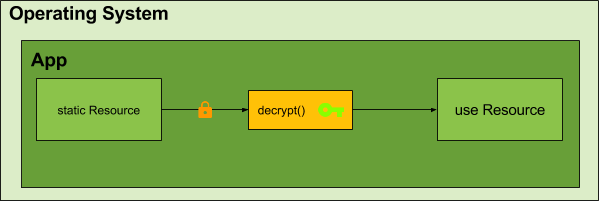
\includegraphics[width=0.8\textwidth]{data/encryptionResource.png}
    \caption{Encrypted resources which have to be decrypted on startup}
    \label{fig:encryptionResource}
\end{figure}

\subsubsection{Action Obfuscator} \label{subsubsectionection:counter-replace-encryption-content-obfuscator}
The second approach is to use encryption as obfuscation.
The idea is to have a method, which is called by each method, to deligate all calls according to an encrypted parameter.
The attacker can try to guess which method call is linked to each method, but when additional encryption for the parameters is applied and decryption is used in the target method, it is very hard to crack the logic without modifying a lot of code.
In order to make it harder to circumvent the encryption of the methods, objects can be encrypted as well.
An abstract presentation of the mechanism can be seen in figure~\ref{fig:encryptionAction}.

\begin{figure}[h]
    \centering
    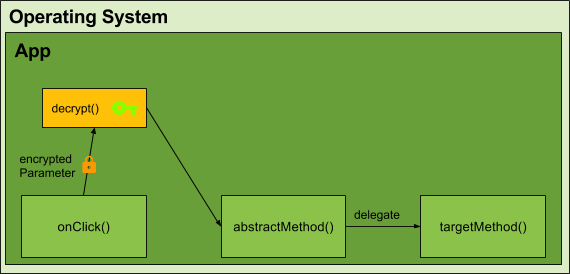
\includegraphics[width=0.8\textwidth]{data/encryptionAction.png}
    \caption{Encrypted actions to obfuscate dependencies}
    \label{fig:encryptionAction}
\end{figure}

\subsubsection{Communication Decryption} \label{section:counter-replace-encryption-content-communication}
The third approach is to use encryption on the server response.
This is an additional security feature which is applied in combination with a content server described in subsection~\ref{section:counter-replace-server}.
When the user does the login on the server, additional unique device specific paramters have be passed as well.
The server generates a cryptographic key which is used for communication is encrypted
\begin{figure}[h]
    \centering
    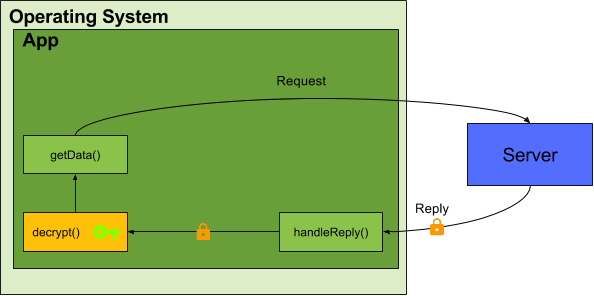
\includegraphics[width=0.8\textwidth]{data/encryptionComm.png}
    \caption{Encrypted communication with a server}
    \label{fig:encryptionComm}
\end{figure}
combined with device specific key, accounts cannot be shared anymore (either hacked or shared libratly)


\url{https://source.android.com/devices/drm.html} store key outside the app and decrypt content, works only for apps which can work with content server, focuses on the security of content on the phone\newline
delivering content is allowed but the deliverer wants to be sure that nobody steals it from the phone


\subsubsection{Encryption} \label{subsubsection:counter-replace-encryption-key}
After applying encrpytion on the application, the handling of the key has to be specified.

\subsubsection{Secure Element} \label{section:counter-replace-encryption-key-online}
\begin{figure}[h]
    \centering
    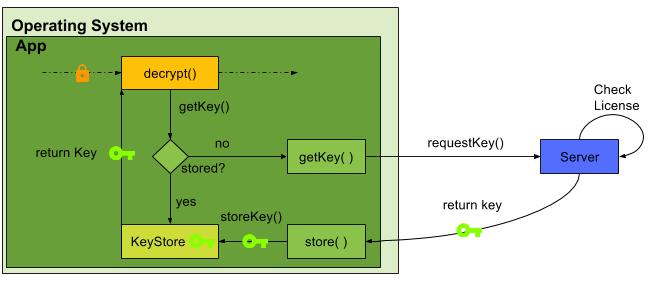
\includegraphics[width=0.8\textwidth]{data/encryptionKeyServer.png}
    \caption{Retrieving the key after successful identification from the server and store it local on device}
    \label{fig:encryptionKeyServer}
\end{figure}

\subsubsection{Secure Element} \label{section:counter-replace-encryption-key-local}

idea: store key at secure place where it is not exposed but delivers decrypted output for an input, best suitable for this task smartcard


can either be mounted in the sdcard slot or using an adapter for the usb interface
accessed over reads and writes to the filesystem
since it has to be small as a sd card and powered by the host system its hardware capabilities are restrained as well \cite{stSe} with power as low as 25MHz complexe calculations would take too much time

simple tasks (beschreiben)

unbestechlich, jedoch boolean abfrage immer crackbar, deswegen andere sachen machen zB verschlüsseln

encrypted strings from the application can be decrypted by the secure element
store property settings on it

encryption key can be stored on

no complexe tasks since low power

\begin{figure}[h]
    \centering
    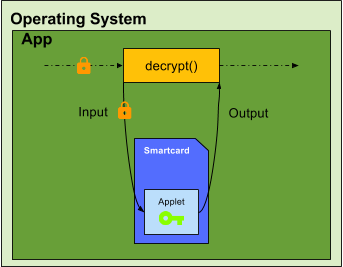
\includegraphics[width=0.8\textwidth]{data/encryptionKeySmart.png}
    \caption{Decryption by using a smartcard}
    \label{fig:encryptionKeySmart}
\end{figure}


same as internet service but extra hardare has to be bought
people are lazy and do not want to have extra hardware
when integrated into phone, it will take a long time until each phone supports it, e.g. was not able to use it on Nexus 6P and Nexus 7, Linux did not recognize it but mass storage was enabled, Nexus7 said OTG available but it did not work
many different implementation fragmentate the market, there is not one single solution to focus on and push for market wide accepted solution
solution which are out there have major security flaws, smartcard itself can be attacked

have problems on their own, nur so sicher wie das secure element
DAP Verification .... normalerweise muss jede Applet, die auf so ein Secure Element/Smartcard etc. kommt mit ner Signatur unterschrieben sein ...
%\url{http://www.win.tue.nl/pinpasjc/docs/Card%20Spec%20v2.1.1%20v0303.pdf}


Waehrend ich Exploits finden konnte, die Dir erw. Zugriff geben, wenn du Applets installieren kannst, u.a.
%\url{https://www.cs.ru.nl/E.Poll/papers/cardis08.pdf}
%\url{http://www.uclouvain.be/crypto/wissec2009/static/13.pdf}​

SD Association
\url{http://www.androidpolice.com/2016/02/22/with-smartsd-the-sd-association-wants-to-adapt-microsd-cards-to-make-mobile-payments/}





TODO:
2) Secure Elements
Bottleneck ist sicherlich die Schnittstelle zu Android und alles was in Android ist, ist prinzipiell unsicher, also auch etwaige Keys. Was jedoch koennte Secure Elements absichern? Ich moechte dich bitten hier Ideen zu erarbeiten, was im Zuge von Kopierschutz,  Verschluesslung etc. mit SEs wirklich sicher gemacht werden koennte. Eine grobe Idee ist z.B. das Signieren von Serveranfragen. Key kennt hier nur das SE und der Server. Android schickt die volle URL mit Parametern und das SE fuegt einen Signaturparameter zu. Vorteil: Ohne das SE kann die App den Server mal nicht mehr nutzen. Jetzt musste man verhindern, dass eine Proxy-App unter Android fuer andere aktiv wird (Stichwort CardSharing). Was koennte man tun? Das ist auch nur ein Idee. Was gibt es sonst noch? Wo koennte es Sinn machen einen sicheren Speicher zu haben?



Since \gls{luckypatcherg} focuses on the manipulation of the license verification libraries, it cannot be used for cracking encryption mechanisms.
Thus implementing encryption protects from \gls{luckypatcherg} and instead the boundaries of encryption apply.
